%%%%%%%%%%%%%%%%%%%%%%%%%%%%%%%%%%%%%%%%%%%%%%%%%%%%%%%%%%%%%%%%%%%%%%%%% 
% 
% Grado en Estadística.
% Universidad de Granada.
% Curso 2017/18.
% 
% 
% Colaboradores:
% Miguel Anguita Ruiz
% 
% Agradecimientos:
% Andrés Herrera (@andreshp) y Mario Román (@M42) por
% las plantillas base.
% 
% Sitio original:
% https://github.com/libreim/apuntesDGIIM/
% 
% Licencia:
% CC BY-NC-SA 4.0 (https://creativecommons.org/licenses/by-nc-sa/4.0/)
% 
%%%%%%%%%%%%%%%%%%%%%%%%%%%%%%%%%%%%%%%%%%%%%%%%%%%%%%%%%%%%%%%%%%%%%%%%% 


% ------------------------------------------------------------------------------
% ACKNOWLEDGMENTS
% ------------------------------------------------------------------------------

%%%%%%%%%%%%%%%%%%%%%%%%%%%%%%%%%%%%%%%%%%%%%%%%%%%%%%%%%%%%%%%%%%%%%%%% 
% Plantilla básica de Latex en Español.
% 
% Autor: Andrés Herrera Poyatos (https://github.com/andreshp) 
% 
% Es una plantilla básica para redactar documentos. Utiliza el paquete fancyhdr
% para darle un estilo moderno pero serio.
% 
% La plantilla se encuentra adaptada al español.
% 
%%%%%%%%%%%%%%%%%%%%%%%%%%%%%%%%%%%%%%%%%%%%%%%%%%%%%%%%%%%%%%%%%%%%%%%%% 

%%%%%%%%%%%%%%%%%%%%%%%%%%%%%%%%%%%%%%%%%%%%%%%%%%%%%%%%%%%%%%%%%%%%%%%%% 
% Plantilla de Trabajo
% Modificación de una plantilla de Latex de Frits Wenneker para adaptarla 
% al castellano y a las necesidades de escribir informática y matemáticas.
% 
% Editada por: Mario Román
% 
% License:
% CC BY-NC-SA 3.0 (http://creativecommons.org/licenses/by-nc-sa/3.0/)
%%%%%%%%%%%%%%%%%%%%%%%%%%%%%%%%%%%%%%%%%%%%%%%%%%%%%%%%%%%%%%%%%%%%%%%%% 

%%%%%%%%%%%%%%%%%%%%%%%%%%%%%%%%%%%%%%%%%%%%%%%%%%%%%%%%%%%%%%%%%%%%%%%%% 
% Short Sectioned Assignment
% LaTeX Template
% Version 1.0 (5/5/12)
% 
% This template has been downloaded from:
% http://www.LaTeXTemplates.com
% 
% Original author:
% Frits Wenneker (http://www.howtotex.com)
% 
% License:
% CC BY-NC-SA 3.0 (http://creativecommons.org/licenses/by-nc-sa/3.0/)
% 
%%%%%%%%%%%%%%%%%%%%%%%%%%%%%%%%%%%%%%%%%%%%%%%%%%%%%%%%%%%%%%%%%%%%%%%%% 


% Tipo de documento y opciones.
%\documentclass[11pt, a4paper, twoside]{article} % Usar para imprimir
\documentclass[11pt, a4paper]{article}

% ---------------------------------------------------------------------------
% PAQUETES
% ---------------------------------------------------------------------------

% Idioma y codificación para Español.
\usepackage[utf8]{inputenc}
\usepackage[spanish, es-tabla, es-lcroman, es-noquoting]{babel}
\selectlanguage{spanish} 
% \usepackage[T1]{fontenc}

% Fuente utilizada.
\usepackage{courier}    % Fuente Courier.
\usepackage{microtype}  % Mejora la letra final de cara al lector.

% Diseño de página.
\usepackage{fancyhdr}   % Utilizado para hacer cabeceras y pies de página.
\usepackage{multirow}

\usepackage{titlesec} 	% Utilizado para hacer títulos propios.
\usepackage{lastpage}   % Referencia a la última página.
\usepackage{extramarks} % Marcas extras. Utilizado en pie de página y cabecera.
\usepackage[parfill]{parskip}    % Crea una nueva línea entre párrafos.
\usepackage{geometry}            % Geometría de las páginas.

% Símbolos y matemáticas.
\usepackage{amssymb, amsmath, amsthm, amsfonts, amscd}
\usepackage{upgreek}
\usepackage{mathrsfs}

\usepackage{mdframed}

% Gráficos

\usepackage{pgf,tikz}
\usepackage{tkz-euclide}
\usetkzobj{all}

% Otros.
\usepackage{enumitem}   % Listas mejoradas.
\usepackage{hyperref}
\usepackage{graphicx}   % Gráficos.
\usepackage[space]{grffile}  % Permitir espacios en rutas de gráficos
\usepackage{xcolor}     % Colores.8

% Fuentes personalizadas

\usepackage[scaled=.85]{newpxtext,newpxmath}
\usepackage[scaled=.85]{FiraSans}
\usepackage[T1]{fontenc}

% Código para ajustar las fuentes matemáticas al estilo del texto
% que le rodea

\DeclareMathVersion{sans}
\SetSymbolFont{operators}{sans}{OT1}{cmbr}{m}{n}
\SetSymbolFont{letters}{sans}{OML}{cmbr}{m}{it}
\SetSymbolFont{symbols}{sans}{OMS}{cmbrs}{m}{n}
\SetMathAlphabet{\mathit}{sans}{OT1}{cmbr}{m}{sl}
\SetMathAlphabet{\mathbf}{sans}{OT1}{cmbr}{bx}{n}
\SetMathAlphabet{\mathtt}{sans}{OT1}{cmtl}{m}{n}
\SetSymbolFont{largesymbols}{sans}{OMX}{iwona}{m}{n}

\DeclareMathVersion{boldsans}
\SetSymbolFont{operators}{boldsans}{OT1}{cmbr}{b}{n}
\SetSymbolFont{letters}{boldsans}{OML}{cmbrm}{b}{it}
\SetSymbolFont{symbols}{boldsans}{OMS}{cmbrs}{b}{n}
\SetMathAlphabet{\mathit}{boldsans}{OT1}{cmbr}{b}{sl}
\SetMathAlphabet{\mathbf}{boldsans}{OT1}{cmbr}{bx}{n}
\SetMathAlphabet{\mathtt}{boldsans}{OT1}{cmtl}{b}{n}
\SetSymbolFont{largesymbols}{boldsans}{OMX}{iwona}{bx}{n}

\newif\IfInSansMode
\let\oldsf\sffamily
\renewcommand*{\sffamily}{\oldsf\mathversion{sans}\InSansModetrue}
\let\oldmd\mdseries
\renewcommand*{\mdseries}{\oldmd\IfInSansMode\mathversion{sans}\fi\relax}
\let\oldbf\bfseries
\renewcommand*{\bfseries}{\oldbf\IfInSansMode\mathversion{boldsans}\else%
   \mathversion{bold}\fi\relax}
\let\oldnorm\normalfont
\renewcommand*{\normalfont}{\oldnorm\InSansModefalse\mathversion{normal}}
\let\oldrm\rmfamily
\renewcommand*{\rmfamily}{\oldrm\InSansModefalse\mathversion{normal}}

% Colores

\definecolor{50}{HTML}{E8F5E9}
\definecolor{300}{HTML}{81C784}
\definecolor{500}{HTML}{4CAF50}
\definecolor{700}{HTML}{388E3C}

% ---------------------------------------------------------------------------
% OPCIONES PERSONALIZADAS
% ---------------------------------------------------------------------------

% Formato de texto.
\linespread{1.3}            % Espaciado entre líneas.
\setlength\parindent{0pt}   % No indentar el texto por defecto.
\setlist{leftmargin=.5in}   % Indentación para las listas.

% Estilo de página.
\pagestyle{fancy}
\fancyhf{}
\geometry{left=3cm,right=3cm,top=3cm,bottom=3cm}   % Márgenes y cabecera.

% Estilo de las cabeceras

\titleformat{\section}
  {\Large\bfseries\sffamily}{\thesection}{1em}{}
\titleformat{\subsection}
  {\large\sffamily}{\thesubsection}{1em}{}
\titleformat{\subsubsection}
  {\sffamily}{\thesubsubsection}{1em}{}

% Estilo de enlaces
\hypersetup{
  % hidelinks = true,   % Oculta todos los enlaces.
  colorlinks = true,   % Muestra todos los enlaces, sin bordes alrededor.
  linkcolor=black,     % Color de enlaces genéricos
  citecolor={blue!50!black},   % Color de enlaces de referencias
  urlcolor={blue!80!black}     % Color de enlaces de URL
}

% Ruta donde buscar gráficos
\graphicspath{{../Recursos/Plantillas/} {Recursos/Plantillas/} {./img/} {Análisis Matemático II/img/}}

% Redefinir entorno de demostración (reducir espacio superior)
% \makeatletter
% \renewenvironment{proof}[1][\proofname] {\vspace{-15pt}\par\pushQED{\qed}\normalfont\topsep6\p@\@plus6\p@\relax\trivlist\item[\hskip\labelsep\it#1\@addpunct{.}]\ignorespaces}{\popQED\endtrivlist\@endpefalse}
% \makeatother

% Aumentar el tamaño del interlineado
\linespread{1.3}

% Permitir salto de página en ecuaciones
\allowdisplaybreaks


% ---------------------------------------------------------------------------
% COMANDOS PERSONALIZADOS
% ---------------------------------------------------------------------------

% Redefinir letra griega épsilon.
\let\epsilon\upvarepsilon

% Valor absoluto: \abs{}
\providecommand{\abs}[1]{\lvert#1\rvert}    

% Fracción grande: \ddfrac{}{}
\newcommand\ddfrac[2]{\frac{\displaystyle #1}{\displaystyle #2}}

% Texto en negrita en modo matemática: \bm{}
\newcommand{\bm}[1]{\boldsymbol{#1}}

% Línea horizontal.
\newcommand{\horrule}[1]{\rule{\linewidth}{#1}}

% Letras de conjuntos
\newcommand{\R}{\mathbb{R}} \newcommand{\N}{\mathbb{N}}

% Sucesiones
\newcommand{\xn}{\{x_n\}}
\newcommand{\fn}{\{f_n\}}

% Letra griega "chi" en línea con el texto
\DeclareRobustCommand{\rchi}{{\Large \mathpalette\irchi\relax}}
\newcommand{\irchi}[2]{\raisebox{0.4\depth}{$#1\chi$}} % inner command, used by \rchi 

% Letra 'omega'
\newcommand{\W}{\Omega}
\newcommand{\w}{\omega}


% ---------------------------------------------------------------------------
% CABECERA Y PIE DE PÁGINA
% ---------------------------------------------------------------------------

\renewcommand{\sectionmark}[1]{%
\markboth{#1}{}}

\renewcommand{\subsectionmark}[1]{%
\markright{#1}{}}

%\addtolength{\headheight}{4ex}
\renewcommand{\headrulewidth}{0pt}

\addtolength{\headwidth}{\marginparsep}
%\addtolength{\headwidth}{\marginparwidth}

\fancypagestyle{section}{%
  \fancyhead{}
  %\addtolength{\headheight}{-10ex}
  %\renewcommand{\headheight}{0pt}%
  %\setlength{\footskip}{-48pt}%
  \fancyfoot[LE,RO]{\Large\sffamily\thepage}
  \renewcommand{\headrulewidth}{0pt}%
  \renewcommand{\footrulewidth}{0pt}%
}

\let\originalsection\section
\RenewDocumentCommand{\section}{som}{%
  \IfBooleanTF{#1}
    {\originalsection*{#3}}
    {\IfNoValueTF{#2}
      {\originalsection{#3}}
      {\originalsection[#2]{#3}}%
    }%
  \thispagestyle{section}%
}

\fancyhead[LE,RO]{\rule[-4ex]{0pt}{2ex}\sffamily\textsl{\rightmark}}
\fancyhead[LO,RE]{\sffamily{\leftmark}}
\fancyfoot[LE,RO]{\Large\sffamily\thepage}



% ---------------------------------------------------------------------------
% ENTORNOS PARA MATEMÁTICAS
% ---------------------------------------------------------------------------

% Nuevo estilo para definiciones.
\newtheoremstyle{definition-style} % Nombre del estilo.
{}               % Espacio por encima.
{}               % Espacio por debajo.
{}                   % Fuente del cuerpo.
{}                   % Identación.
{\bf\sffamily}                % Fuente para la cabecera.
{.}                  % Puntuación tras la cabecera.
{.5em}               % Espacio tras la cabecera.
{\thmname{#1}\thmnumber{ #2}\thmnote{ (#3)}}     % Especificación de la cabecera (actual: nombre en negrita).

% Nuevo estilo para notas.
\newtheoremstyle{remark-style} 
{10pt}                
{10pt}                
{}                   
{}                   
{\itshape \sffamily}          
{.}                  
{.5em}               
{}                  

% Nuevo estilo para teoremas y proposiciones.
\newtheoremstyle{theorem-style}
{}                
{}                
{}           
{}                  
{\bfseries \sffamily}             
{.}                
{.5em}           
{\thmname{#1}\thmnumber{ #2}\thmnote{ (#3)}}

% Nuevo estilo para ejemplos.
\newtheoremstyle{example-style}
{10pt}                
{10pt}                
{}                  
{}                   
{\bf \sffamily}              
{}                 
{.5em}               
{\thmname{#1}\thmnumber{ #2.}\thmnote{ #3.}}  

% Nuevo estilo para la demostración
%\renewenvironment{proof}{{\itshape \sffamily Demostración \\}}{\hspace*{\fill}\qed}

\makeatletter
\renewenvironment{proof}[1][\proofname] {\par\pushQED{\qed}\normalfont\topsep6\p@\@plus6\p@\relax\trivlist\item[\hskip\labelsep\itshape\sffamily#1\@addpunct{.}]\ignorespaces}{\popQED\endtrivlist\@endpefalse}
\makeatother

% Configuración general de mdframe, los estilos de los teoremas, etc
\mdfsetup{skipabove=12pt,skipbelow=12pt,innertopmargin=12pt,innerbottommargin=4pt}

% Creamos los 'marcos' de los estilos

\mdfdefinestyle{nth-frame}{
	linewidth=2pt, %
	linecolor= 500, % 
	%linecolor=black,
	topline=false, %
	bottomline=false, %
	rightline=false,%
	leftmargin=0pt, %
	innerleftmargin=1em, % 
	rightmargin=0pt, %
	innerrightmargin=0pt, % % 
	%splittopskip=\topskip, %
	%splitbottomskip=\topskip, %
}% 

\mdfdefinestyle{nprop-frame}{
	linewidth=2pt, %
	linecolor= 300, %
	%linecolor= gray, 
	topline=false, %
	bottomline=false, %
	rightline=false,%
	leftmargin=0pt, %
	innerleftmargin=1em, %
	innerrightmargin=0em, 
	rightmargin=0pt, %
	%splittopskip=\topskip, %
	%splitbottomskip=\topskip, %
}%       

\mdfdefinestyle{ndef-frame}{
	linewidth=2pt, %
	linecolor= 300, % 
	%linecolor= gray!50,
	backgroundcolor= 50,
	%backgroundcolor= gray!5,
	topline=false, %
	bottomline=false, %
	rightline=false,%
	leftmargin=0pt, %
	innerleftmargin=1em, %
	innerrightmargin=1em, 
	rightmargin=0pt, % 
	innertopmargin=1.5em,%
	innerbottommargin=1em, % 
	splittopskip=\topskip, %
	%splitbottomskip=\topskip, %
}% 

\mdfdefinestyle{ejemplo-frame}{
	linewidth=0pt, %
	linecolor= 300, % 
	%backgroundcolor= 50,
	leftline=false, %
	rightline=false, %
	leftmargin=0pt, %
	innerleftmargin=1.5em, %
	innerrightmargin=1.5em, 
	rightmargin=0pt, % 
	innertopmargin=0em,%
	innerbottommargin=0em, % 
	splittopskip=\topskip, %
	%splitbottomskip=\topskip, %
}%                

% Asignamos los marcos a los estilos

\surroundwithmdframed[style=nth-frame]{nth}
\surroundwithmdframed[style=nprop-frame]{nprop}
\surroundwithmdframed[style=nprop-frame]{ncor}
\surroundwithmdframed[style=ndef-frame]{ndef}
\surroundwithmdframed[style=ejemplo-frame]{ejemplo}
                 
% Asignamos los estilos definidos anteriormente a los entornos correspondientes
% Teoremas, proposiciones y corolarios.
\theoremstyle{theorem-style}
\newtheorem{nth}{Teorema}[section]
\newtheorem{nprop}{Proposición}[section]
\newtheorem{ncor}{Corolario}[section]
\newtheorem{lema}{Lema}[section]
% Definiciones.
\theoremstyle{definition-style}
\newtheorem{ndef}{Definición}[section]
\newtheorem{ejer}{Ejercicio}[section]

% Notas.
\theoremstyle{remark-style}
\newtheorem*{nota}{Nota}
\newtheorem*{sol}{Solución}


% Ejemplos.
\theoremstyle{example-style}
\newtheorem{ejemplo}{Ejemplo}[section]



% Listas ordenadas con números romanos (i), (ii), etc.
\newenvironment{nlist}
{\begin{enumerate}
    \renewcommand\labelenumi{(\emph{\roman{enumi})}}}
  {\end{enumerate}}

% División por casos con llave a la derecha.
\newenvironment{rcases}
{\left.\begin{aligned}}
    {\end{aligned}\right\rbrace}


% ---------------------------------------------------------------------------
% PÁGINA DE TÍTULO
% ---------------------------------------------------------------------------

% Título del documento.
\newcommand{\subject}{Prácticas de ordenador: distribuciones discretas y continuas unidimensionales}

% Autor del documento.
\newcommand{\docauthor}{Miguel Anguita Ruiz}

% Título
\title{
  \normalfont \normalsize 
  \textsc{Universidad de Granada} \\ [25pt]    % Texto por encima.
  \textsc{Grado en Estadística} \\ [25pt]    % Texto por encima.
  \horrule{0.5pt} \\[0.4cm] % Línea horizontal fina.
  \huge \sffamily\subject\\ % Título.
  \horrule{2pt} \\[0.5cm] % Línea horizontal gruesa.
}

% Autor.
\author{\Large\sffamily{\docauthor}}

% Fecha.
\date{\vspace{-1.5em} \normalsize \sffamily Curso 2017/18}



% ---------------------------------------------------------------------------
% COMIENZO DEL DOCUMENTO
% ---------------------------------------------------------------------------

\begin{document}

\maketitle  % Título.
\vfill
\begin{center}
  %\includegraphics{by-nc-sa.pdf}  % Licencia.
\end{center}
\newpage
\tableofcontents    % Índice
\newpage


% --------------------------------------------------------------------------------
% Introducción.
% --------------------------------------------------------------------------------

\section{Práctica 1}

\begin{ejer}.
\\

Calcular, para cada una de las distribuciones especificadas en las filas, los valores de probabilidades, percentiles y rango intercuartílico solicitados en las columnas de las siguientes tablas. \\ Sea mi DNI = 77149477, la tabla asociada es la siguiente:  

\begin{table}[htbp]
	\begin{center}
		\begin{tabular}{|l|l|l|l|l|l|}
			\hline
			 & P(X=1) & P(X $ \le$ 2) & P(X > 2) & Percentiles 0.05, 0.1, 0.65 & Rango intercuartílico \\
			\hline \hline
			B(5,0.3) & 0.36015 & 0.83692 & 0.16308 & (0,0,2) & 1 \\ \hline
			P(1.5) & 0.3346952 & 0.8088468 & 0.1911532 & (0,0,2) & 1 \\ \hline
			BN(4,0.3) & 0.02268 & 0.07047 & 0.92953 & (2,3,11) & 7\\ \hline
			G(0.5) & 0.25 & 0.875 & 0.125 & (0,0,1) & 1\\ \hline
			H(11,3,5) & 0.4545455 & 0.9393939 & 0.06060606 & (0,0,2) & 1\\ \hline
		\end{tabular}
	\end{center}
\end{table}

\begin{table}[htbp]
	\begin{center}
		\begin{tabular}{|l|l|l|l|l|l|}
			\hline
			& $f(4.3)$ & P(X $ \le$ 5.3) & P(X > 1) & Percentiles 0.25, 0.5, 0.55 & Rango intercuartílico \\
			\hline \hline
			N(4.4,1.4) & 0.3359657 & 0.7765636 & 0.9979704 & (3.601933,4.4,5.198067) & 1.596134 \\ \hline
			Exp(0.85) & 0.007474152 & 0.9980409 & 0.3083652 & (0.2445298,0.5891751,0.6787315) & 0.9338204 \\ \hline
		\end{tabular}
	\end{center}
\end{table}

\begin{table}[htbp]
	\begin{center}
		\begin{tabular}{|l|l|l|l|l|l|}
			\hline
			& $f(0.35)$ & P(X $ \le$ 0.95) & P(X > 0.7) & Percentiles 0.25, 0.5, 0.55 & Rango intercuartílico \\
			\hline \hline
			$\Gamma(1.9,1.1)$ & 0.2453359 & 0.2405288 & 0.8453424 & (0.9771061,1.736963,1.913223) & 1.846206 \\ \hline
			Be(1.9,1.1) & 0.8139028 & 0.928102 & 0.4529392 & (0.4565206,0.6659588,0.7020887) & 0.3800205 \\ \hline
		\end{tabular}
	\end{center}
\end{table}

Los comandos en R usados han sido los siguientes:

\begin{enumerate}
	\item Para B(5,0.3):
			\begin{itemize}
				\item dbinom(1,5,0.3)
				
				\item pbinom(2,5,0.3)
				
				\item pbinom(2,5,0.3,lower.tail = F)
				
				\item qbinom(0.05,5,0.3)
				
				\item qbinom(0.1,5,0.3)
				
				\item qbinom(0.65,5,0.3)
				
				\item qbinom(0.75,5,0.3)-qbinom(0.25,5,0.3)
			\end{itemize}
	\item Para P(1.5):
	\begin{itemize}
		\item dpois(1,1.5)
		
		\item ppois(2,1.5)
		
		\item ppois(2,1.5,lower.tail = F)
		
		\item qpois(0.05,1.5)
		
		\item qpois(0.1,1.5)
		
		\item qpois(0.65,1.5)
		
		\item qpois(0.75,1.5)-qpois(0.25,1.5)
	\end{itemize}
	\item Para BN(4,0.3):
	\begin{itemize}
		\item dnbinom(1,4,0.3)
		
		\item pnbinom(2,4,0.3)
		
		\item pnbinom(2,4,0.3,lower.tail = F)
		
		\item qnbinom(0.05,4,0.3)
		
		\item qnbinom(0.1,4,0.3)
		
		\item qnbinom(0.65,4,0.3)
		
		\item qnbinom(0.75,4,0.3)-qnbinom(0.25,4,0.3)
	\end{itemize}
	\item Para G(0.5):
	\begin{itemize}
		\item dgeom(1,0.5)
		
		\item pgeom(2,0.5)
		
		\item pgeom(2,0.5,lower.tail = F)
		
		\item qgeom(0.05,0.5)
		
		\item qgeom(0.1,0.5)
		
		\item qgeom(0.65,0.5)
		
		\item qgeom(0.75,0.5)-qgeom(0.25,0.5)
	\end{itemize}
	\item Para H(11,3,5):
	\begin{itemize}
	
		\item dhyper(1,5,6,3)
	
		\item phyper(2,5,6,3)
	
		\item phyper(2,5,6,3, lower.tail = F)
	
		\item qhyper(0.05,5,6,3)
	
		\item qhyper(0.1,5,6,3)
	
		\item qhyper(0.65,5,6,3)
	
		\item qhyper(0.75,5,6,3)-qhyper(0.25,5,6,3) 
	\end{itemize}
	\item Para N(4.4,1.4):
	\begin{itemize}
		\item dnorm(4.3,mean=4.4,sd=sqrt(1.4))
		
		\item pnorm(5.3,mean=4.4,sd=sqrt(1.4))
		
		\item pnorm(1,mean=4.4,sd=sqrt(1.4),lower.tail = F)
		
		\item qnorm(0.25,mean=4.4,sd=sqrt(1.4))
		
		\item qnorm(0.5,mean=4.4,sd=sqrt(1.4))
		
		\item qnorm(0.55,mean=4.4,sd=sqrt(1.4))
		
		\item qnorm(0.75,mean=4.4,sd=sqrt(1.4))-qnorm(0.25,mean=4.4,sd=sqrt(1.4))
	\end{itemize}
	\item Para Exp(0.85):
		\begin{itemize}
			\item dexp(4.3,1/0.85)
			
			\item pexp(5.3,1/0.85)
			
			\item pexp(1,1/0.85,lower.tail = F)
			
			\item qexp(0.25,1/0.85)
			
			\item qexp(0.5,1/0.85)
			
			\item qexp(0.55,1/0.85)
			
			\item qexp(0.75,1/0.85)-qexp(0.25,1/0.85)
		\end{itemize}
	\item Para $\Gamma(1.9,1.1)$:
		\begin{itemize}
			\item dgamma(0.35,shape=1.9,scale=1.1)
			
			\item pgamma(0.95,shape=1.9,scale=1.1)
			
			\item pgamma(0.7,shape=1.9,scale=1.1,lower.tail = F)
			
			\item qgamma(0.25,shape=1.9,scale=1.1)
			
			\item qgamma(0.5,shape=1.9,scale=1.1)
			
			\item qgamma(0.55,shape=1.9,scale=1.1)
			
			\item qgamma(0.75,shape=1.9,scale=1.1)-qgamma(0.25,shape=1.9,scale=1.1)
		\end{itemize}
		\item Para Be(1.9,1.1):
		\begin{itemize}
			\item dbeta(0.35,shape1 = 1.9,shape2 = 1.1)
			
			\item pbeta(0.95,shape1 = 1.9,shape2 = 1.1)
			
			\item pbeta(0.7,shape1 = 1.9,shape2 = 1.1,lower.tail = F)
			
			\item qbeta(0.25,shape1 = 1.9,shape2 = 1.1)
			
			\item qbeta(0.5,shape1 = 1.9,shape2 = 1.1)
			
			\item qbeta(0.55,shape1 = 1.9,shape2 = 1.1)
			
			\item qbeta(0.75,shape1 = 1.9,shape2 = 1.1)-qbeta(0.25,shape1 = 1.9,shape2 = 1.1) \\ 
		\end{itemize}
	
\end{enumerate}




\end{ejer}

\begin{ejer}

Representa gráficamente la función de densidad y la función de distribución de una distribución Normal de media 10 y desviación típica 4, personaliza los gráficos a tu gusto y añádelos al documento a entregar.

\begin{sol}
	
.\\

Las funciones de densidad y distribución de una distribución normal de media 10 y desviación típica 4, son, respectivamente, las siguientes:
	
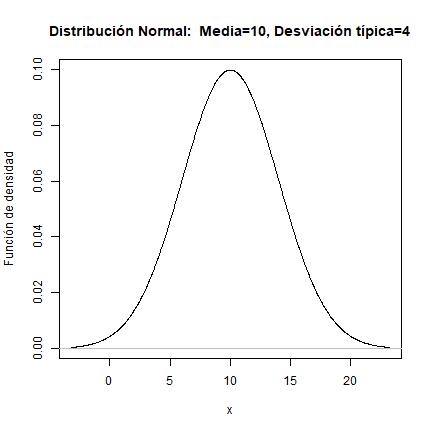
\includegraphics[]{FDensidad.jpg}

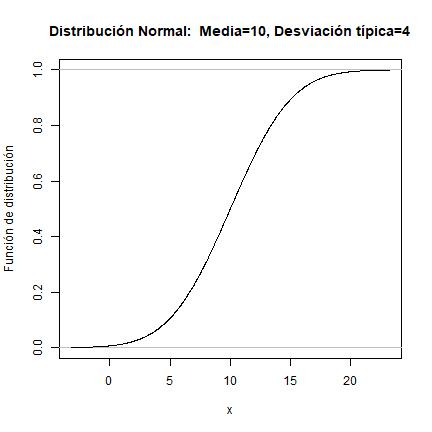
\includegraphics[]{FDistribucion.jpg}
El código usado ha sido el siguiente:

\begin{enumerate}
	\item Para la función de densidad:
		\begin{itemize}
			\item local(\{\ \\
				.x <- seq(-3.162, 23.162, length.out=1000)  
				plotDistr(.x, dnorm(.x, mean=10, sd=4), cdf=FALSE, xlab="x", ylab="Función de densidad", 
				main=paste("Distribución Normal:  Media=10, Desviación típica=4")) \\
			\}\ )
		\end{itemize}
	\item Para la función de distribución:
		\begin{itemize}
			\item local(\{\
				.x <- seq(-3.162, 23.162, length.out=1000)  
				plotDistr(.x, pnorm(.x, mean=10, sd=4), cdf=TRUE, xlab="x", ylab="Función de distribución", 
				main=paste("Distribución Normal:  Media=10, Desviación típica=4")) \\
			\}\ )
		\end{itemize}
\end{enumerate}
 
	
	
	
	
	
	
	

\end{sol}








\end{ejer}

% FIN DEL DOCUMENTO
% ---------------------------------------------------------------------------

\end{document}